% NAMER technical preprint. Self-contained: bibliography and vector figures
% are embedded. Compile twice with pdflatex, or use latexmk -pdf.
% Author metadata is deliberately centralized for easy editing.
\documentclass[11pt,letterpaper]{article}
\usepackage[T1]{fontenc}
\usepackage[utf8]{inputenc}
\usepackage{lmodern}
\usepackage[margin=0.94in]{geometry}
\usepackage{microtype}
\usepackage{amsmath,amssymb,mathtools}
\usepackage{booktabs,array,tabularx}
\usepackage{graphicx}
\usepackage{flafter}
\usepackage{tikz}
\usetikzlibrary{arrows.meta,positioning,calc}
\usepackage[numbers,sort&compress]{natbib}
\usepackage{caption}
\usepackage{xurl}
\usepackage[hidelinks]{hyperref}
\usepackage{fancyhdr}
\usepackage{enumitem}
\usepackage{needspace}
\usepackage{placeins}
\newcommand{\paperauthor}{Kenneth Hurley}
\newcommand{\paperaffiliation}{Genius Ventures}
\newcommand{\paperdate}{September 21, 2026}
\newcommand{\commit}{9eb068520b6e5fcf3ff39e13291dedd3f88e0015}
\newcommand{\shortcommit}{9eb0685}
\newcommand{\sat}{\operatorname{sat}}
\newcommand{\clamp}{\operatorname{clamp}}
\newcommand{\diag}{\operatorname{diag}}
\newcommand{\R}{\mathbb{R}}
\newcommand{\one}{\mathbf{1}}
\newcommand{\vcol}{\widehat{V}}
\newcommand{\rasterv}{\overline{V}}
\newcommand{\code}[1]{\texttt{#1}}
\newcolumntype{Y}{>{\raggedright\arraybackslash}X}
\newcolumntype{C}[1]{>{\centering\arraybackslash}p{#1}}
\captionsetup{font=small,labelfont=bf,skip=7pt}
\setlength{\parskip}{3pt}
\setlength{\parindent}{1.1em}
\setlength{\emergencystretch}{2em}
\raggedbottom
\setlength{\headheight}{14pt}
\renewcommand{\arraystretch}{1.16}
\setlist{nosep,leftmargin=1.6em}
\setcounter{topnumber}{3}
\setcounter{bottomnumber}{2}
\setcounter{totalnumber}{5}
\renewcommand{\topfraction}{0.95}
\renewcommand{\bottomfraction}{0.9}
\renewcommand{\textfraction}{0.05}
\renewcommand{\floatpagefraction}{0.85}
\pagestyle{fancy}
\fancyhf{}
\fancyhead[L]{\small NAMER: Material Decomposition and Encoding}
\fancyhead[R]{\small Technical preprint}
\fancyfoot[C]{\thepage}
\renewcommand{\headrulewidth}{0.3pt}
\hypersetup{pdftitle={NAMER: Geometry-Aware Material Decomposition and Compact Encoding for Real-Time Rendering},pdfauthor={Kenneth Hurley},pdfsubject={AO extraction and separation, mesh-aware compaction, and planned metallic, emissive, and palette controls},pdfkeywords={real-time rendering, material decomposition, ambient occlusion, metallic extraction, emissive extraction, vertex colors, palette recoloring}}
\title{\vspace{-1.5em}\textbf{NAMER: Geometry-Aware Material Decomposition and Compact Encoding for Real-Time Rendering}}
\author{\paperauthor\\[3pt]\small\paperaffiliation}
\date{\small\paperdate\quad---\quad Revised draft, version 2}

\begin{document}
\maketitle
\thispagestyle{plain}

\begin{abstract}
NAMER is a material decomposition and encoding system for real-time rendering. Rather than treating conversion as texture packing alone, it separates the acquisition of surface signals, the removal or redistribution of baked appearance, and the storage of an editable runtime material. The Unity implementation reuses authored ambient occlusion (AO), synthesizes missing AO from mesh geometry, and retains an image-space extraction path for direct use. A controlled division separates an AO term from base color before fitting broad color variation to quantized mesh vertex colors. Detail outside that mesh representation can remain in a floating-point residual or influence roughness through a signed scalar transfer. A single RGBA8 surface map holds normal coordinates, AO, six-bit roughness, and binary metallic and emissive masks. We formalize these stages, their ordering, and their reconstruction conditions, and characterize their storage and numerical behavior. Planned extensions estimate metallic and emissive masks and associated material-level values while retaining the compact layout, then map color tables onto the separated appearance for recoloring and hand-painted-style art direction. The result is a framework for material extraction, simplification, and control, with implemented mechanisms distinguished from proposed estimators. The reported numerical evidence consists of analytical storage calculations and reproducible scalar checks; rendered-quality and performance evaluation remain future work.
\end{abstract}
\vspace{2pt}
\noindent\textbf{Keywords:} material decomposition; ambient occlusion extraction; vertex colors; roughness transfer; metallic and emissive estimation; compact materials; palette editing.

\section{Introduction}
A source texture can contain several kinds of information at once: broad surface color, fine painted detail, darkening near geometric recesses, and highlights or luminous features baked into the image. A material conversion system must decide which information belongs in color, which belongs in a lighting or surface-response parameter, and which should remain under artistic control. Compressing existing maps does not, by itself, make those distinctions.

NAMER addresses this problem as a sequence of \emph{extraction, separation, representation, and recomposition}. Extraction obtains a material signal from an authored map, geometry, or an image-based estimate. Separation removes or isolates a selected contribution from the color target. Representation allocates the resulting information to mesh attributes, compact surface fields, and optional residuals. Recomposition assembles these quantities for runtime shading. The implementation provides this workflow entirely within the Unity Editor~\cite{namer2026}.

Ambient occlusion is central to this sequence. NAMER preserves an authored AO map when one exists and otherwise supports a geometry bake. It also contains a luminance-based extraction path, retained for direct callers rather than used as the automatic default. An adjustable AO division changes the color target before the mesh fit. This permits broad color to be represented independently of selected recess darkening, while the AO field remains available for recomposition and lighting. Obtaining an AO field and separating that field from color are distinct operations; neither should be reduced to a description of the blue storage channel.

The color representation then fits broad variation to the mesh's piecewise-linear vertex basis. An optional HDR residual retains detail that does not fit. Alternatively, or additionally, a signed scalar component of removed detail can modulate roughness. This \emph{detail-to-roughness transfer} deliberately changes how the surface responds to lighting. It is an appearance-design operation rather than an exact recovery of the original reflectance function.

Metallic and emissive extraction extend the same framework. The current format already has spatial mask capacity, and the implementation imports metallic data and uses a material-level emission signal. The planned work concerns how to obtain missing masks and associated values, not merely how to reserve bits for them. The intended compact controls pair a metallic mask with a material-level metallic multiplier, and an emissive mask with one shared emission color. These estimates can remain separate from subsequent palette edits.

The paper contributes a formulation of this combined material workflow; a detailed account of AO acquisition and separation, vertex-color fitting, residual recovery, and roughness transfer; and a prospective design for metallic/emissive extraction and color-table control within the compact representation. The contribution lies in their integration and information allocation. AO baking, interpolated vertex color, least-squares fitting, and palette editing have established precedents.

\paragraph{Scope and evidence.}
The implementation description is pinned to version 0.1.0 at commit \code{\shortcommit} of NAMER Unity~\cite{namer2026}. Proposed metallic/emissive estimators and color-table operations are identified as extensions rather than completed features. Numerical results are analytical calculations and independently executed scalar checks, not Unity test results, GPU measurements, or a perceptual study.

\section{Related Work}
\paragraph{Mesh-associated color.}
Gouraud shading established the use of interpolated vertex quantities for smooth appearance~\cite{gouraud1971}. NAMER uses that interpolation basis to represent fitted material color, rather than claiming a new interpolation method. Mesh Colors~\cite{yuksel2010} stores color samples in association with mesh vertices, edges, and faces, allowing detail beyond a simple per-vertex field. NAMER instead emphasizes reuse of the existing vertex budget, accepting the spatial limitations of that choice and retaining a residual when desired.

\paragraph{Normal representations and texture coding.}
Cigolle et al.~\cite{cigolle2014} survey compact unit-vector representations, including octahedral encodings. NAMER's current normal format uses a barycentric projection of nonnegative normal-map texels and a quadratic inverse. Although the repository calls this octahedral encoding, it is not the conventional signed, folded octahedral map. Its domain restriction must be considered separately from the properties of the encodings in that survey.

Hardware block compression is also a distinct comparison. BC7 encodes a $4\times4$ block in 16 bytes, or one byte per texel~\cite{bc7}. Packing material channels into an uncompressed RGBA8 texture is not equivalent to block-compressing that texture. Random-Access Neural Compression of Material Textures~\cite{vaidyanathan2023} takes another approach, learning a compact representation and decoder for jointly compressed material textures. NAMER requires no learned material decoder, but this architectural difference does not establish superior rate--distortion performance.

\paragraph{Recoloring and painterly appearance.}
Palette-based Photo Recoloring~\cite{chang2015} demonstrates image recoloring through editable palettes. The proposed NAMER extension relocates such control to a mesh-associated material representation; palette editing itself is established prior work. Likewise, painterly rendering can involve explicit stroke placement, shape, and scale, as in Hertzmann~\cite{hertzmann1998}. A color-table transformation alone does not synthesize brush strokes. The proposed hand-painted-style workflow concerns coherent color design and simplified material detail, with stroke synthesis outside the current scope.


\paragraph{Occlusion, intrinsic appearance, and material semantics.}
Precomputed ambient occlusion estimates environmental visibility from geometry~\cite{pharr2004ao}. Cosine-weighted hemisphere sampling provides the corresponding diffuse-accessibility estimator~\cite{pbrt2023sampling}. NAMER uses this established geometry signal within a larger color-separation and encoding workflow; it does not claim a new definition of AO. In contrast, inferring reflectance and illumination from image appearance requires assumptions or additional evidence, as illustrated by SIRFS~\cite{barron2015}. This distinction matters both to luminance-based AO extraction and to future metallic/emissive estimation. Material specifications such as glTF separate metallic response, occlusion, and emitted color~\cite{gltf2}; NAMER targets a restricted, compact representation of those roles rather than treating bright or dark pixels as physical labels.

\section{Representation and Surface Format}

\subsection{Separate extraction from the storage contract}
The working material description is a set of fields
\begin{equation}
\mathcal M(u)=\{C_0(u),\,n(u),\,a(u),\,r(u),\,m(u),\,\mathbf e(u)\},
\label{eq:materialfields}
\end{equation}
where $a=1$ denotes no occlusion, $m$ is metallic response, and $\mathbf e$ is emitted color in a specified linear working space. These fields can have different origins and need not all be inferred. Table~\ref{tab:status} separates current extraction and conversion from the planned work. Continuous editor-time estimates do not imply continuous per-texel storage: the runtime layout deliberately quantizes some fields to masks.

\begin{table}[htbp]
\centering
\caption{Component scope at the pinned commit and the planned extensions. ``Implemented'' denotes inspected code, not a new benchmark result.}
\label{tab:status}
\small
\begin{tabularx}{\linewidth}{@{}>{\raggedright\arraybackslash}p{0.16\linewidth}Y >{\raggedright\arraybackslash}p{0.29\linewidth}@{}}
\toprule
Component & Acquisition or processing & Status \\
\midrule
Normal & Imported normal reconstruction and two-coordinate encoding & Implemented \\
AO & Authored-map reuse; geometry bake; controlled color separation & Implemented; automatic path \\
Image-space AO & Luminance, low-pass, relative-intensity estimate & Implemented; direct callers only \\
Base color & Linearization, vertex fit, optional HDR residual & Implemented \\
Roughness & Authored data, signed removed-detail or Sobel-derived signal & Implemented; authored-data precedence \\
Metallic & Authored map or scalar, then binary threshold & Import implemented; missing-signal estimation planned \\
Emissive & Uniform emission signal and shared emission color & Uniform path implemented; spatial extraction planned \\
Color tables & Palette-based editing of separated appearance & Planned \\
\bottomrule
\end{tabularx}
\end{table}

\subsection{Representation modes}
Let $C(u)\in\R^3$ denote the source linear base-color field at UV coordinate $u$. Let $C_0(u)$ be the normalized color target after optional occlusion factorization. For a triangle with barycentric coordinates $\lambda_i(u)$ and stored vertex colors $c_i$, the ideal runtime color field is
\begin{equation}
\vcol(u)=\sum_{i=1}^{3}\lambda_i(u)c_i,
\qquad \sum_i\lambda_i(u)=1.
\label{eq:vertexfield}
\end{equation}
NAMER combines this field with a packed surface map $S(u)$ and, optionally, a multiplicative residual $R(u)$. Table~\ref{tab:modes} distinguishes the generated assets in each mode. ``One texture'' refers to the generated, nonconstant material texture asset, not to the number of shader sampling instructions or to all textures used by scene lighting.

\begin{table}[htbp]
\centering
\caption{Material modes. The table excludes shared engine textures, constant defaults, and an independently assigned roughness-offset map.}
\label{tab:modes}
\begin{tabularx}{\linewidth}{@{}p{0.23\linewidth}Y C{1.05in}@{}}
\toprule
Mode & Color representation & Generated maps \\
\midrule
Packed surface only & Base-color texture; neutral vertex multiplier & Base + surface \\
Vertex projection & Fitted vertex RGB; identity color residual & Surface \\
Vertex + residual & Fitted vertex RGB multiplied by an HDR residual & Surface + residual \\
\bottomrule
\end{tabularx}
\end{table}


\begin{figure}[htbp]
\centering
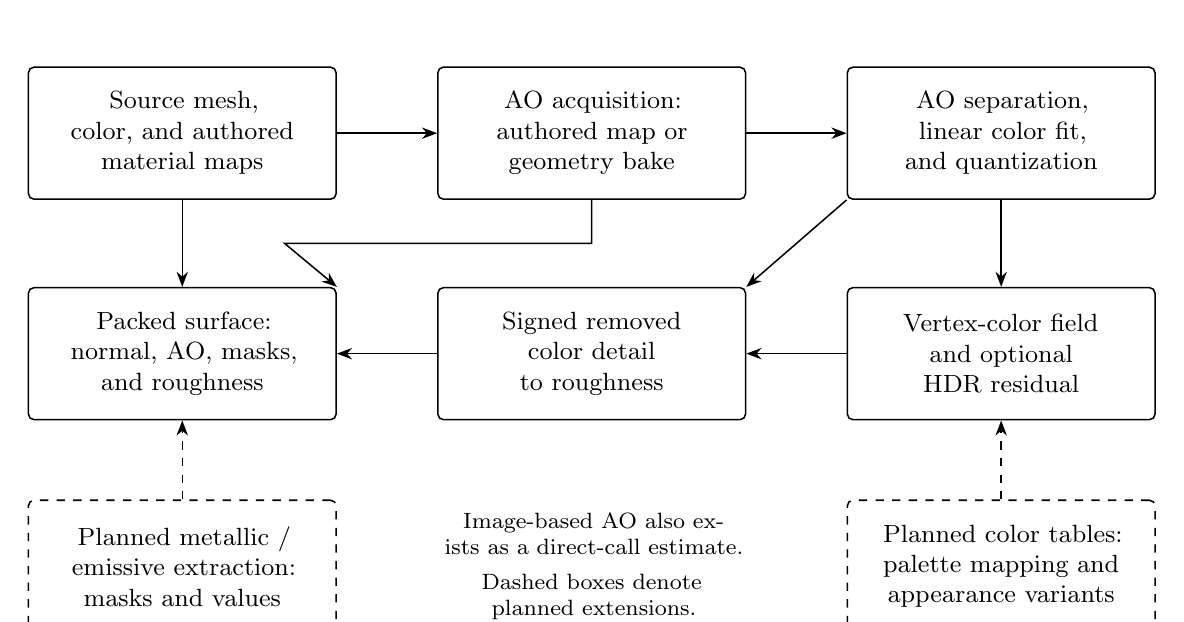
\begin{tikzpicture}[font=\small,>=Stealth,
 box/.style={draw,rounded corners=2pt,align=center,minimum height=0.66in,text width=1.40in,inner sep=5pt},
 future/.style={box,dashed},every path/.style={line width=0.55pt}]
\node[box] (src) at (0,0) {Source mesh,\\color, and authored\\material maps};
\node[box] (ao) at (5.2,0) {AO acquisition:\\authored map or\\geometry bake};
\node[box] (fit) at (10.4,0) {AO separation,\\linear color fit,\\and quantization};
\node[box] (surface) at (0,-2.8) {Packed surface:\\normal, AO, masks,\\and roughness};
\node[box] (detail) at (5.2,-2.8) {Signed removed\\color detail\\to roughness};
\node[box] (vertex) at (10.4,-2.8) {Vertex-color field\\and optional\\HDR residual};
\node[future] (me) at (0,-5.5) {Planned metallic /\\emissive extraction:\\masks and values};
\node[future] (pal) at (10.4,-5.5) {Planned color tables:\\palette mapping and\\appearance variants};
\draw[->] (src) -- (ao);
\draw[->] (ao) -- (fit);
\draw[->] (fit) -- (vertex);
\draw[->] (fit.south west) -- (detail.north east);
\draw[->] (vertex) -- (detail);
\draw[->] (detail) -- (surface);
\draw[->] (src) -- (surface);
\draw[->] (ao.south) -- (5.2,-1.4) -- (1.3,-1.4) -- (surface.north east);
\draw[->,dashed] (me) -- (surface);
\draw[->,dashed] (pal) -- (vertex);
\node[align=center,font=\footnotesize,text width=1.9in] at (5.2,-5.5) {Image-based AO also exists as a direct-call estimate.\\[3pt]Dashed boxes denote planned extensions.};
\end{tikzpicture}
\caption{Material-level information flow. AO is acquired and separated before color fitting; it is not merely packed after the fit. Future metallic/emissive extraction supplies semantic masks and shared values, while color tables edit appearance independently. The diagram is a method schematic, not a rendering result.}
\label{fig:pipeline}
\end{figure}

Figure~\ref{fig:preview} shows a representative synchronized editor preview of a source material and its NAMER-converted counterpart. The image is included as a qualitative sanity check of the conversion workflow rather than as a controlled perceptual benchmark; quantitative image-quality claims require the evaluation protocol described in Section~\ref{sec:evaluation}.

\begin{figure}[htbp]
\centering
\includegraphics[width=\linewidth]{figures/preview-before-after.png}
\caption{Representative NAMER before/after preview from the Unity editor. The left pane shows the source material and the right pane shows the converted NAMER material in the synchronized preview. The close visual agreement in this single example is illustrative only; it is not an aggregate fidelity measurement or a substitute for controlled evaluation.}
\label{fig:preview}
\end{figure}

\subsection{Packed channels}
Each surface texel is stored as linear RGBA8, with the allocation shown in Figure~\ref{fig:bits}. Red and green store two normal coordinates, blue stores ambient occlusion, and alpha stores binary metallic and emissive fields plus six-bit roughness. Writing $\sat(x)=\clamp(x,0,1)$, for normalized roughness $r\in[0,1]$,
\begin{align}
M &= \mathbf{1}[m>0.5], & E &= \mathbf{1}[e>0.1],\\
q_r &= \clamp(\lfloor63r\rfloor,0,63), &
A &=128M+64E+q_r.
\label{eq:pack}
\end{align}
The stored alpha is $A/255$. After recovering the byte, the decoder evaluates
\begin{equation}
\widehat r=\frac{A\mathbin{\&}63}{63},
\qquad \text{smoothness}=1-\widehat r.
\label{eq:roughdecode}
\end{equation}
There are 64 representable roughness values, including both endpoints. Ignoring floating-point behavior at bin boundaries, floor quantization gives $0\le r-\widehat r<1/63$ for $r<1$, with exact representation at $r=1$.

\begin{figure}[htbp]
\centering
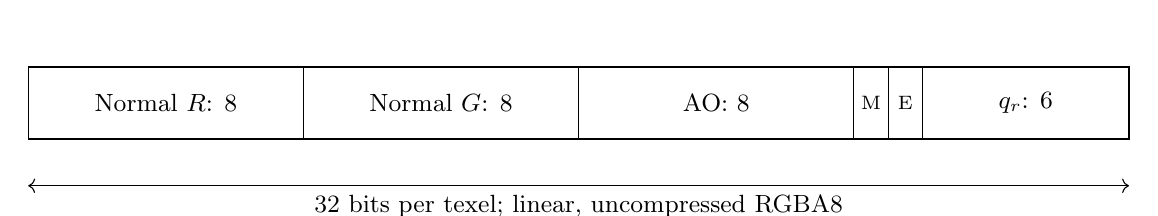
\begin{tikzpicture}[x=0.172in,y=0.36in,font=\small]
\draw (0,0) rectangle (32,1);
\foreach \x in {8,16,24,25,26} {\draw (\x,0)--(\x,1);}
\node at (4,0.5) {Normal $R$: 8};
\node at (12,0.5) {Normal $G$: 8};
\node at (20,0.5) {AO: 8};
\node[font=\scriptsize] at (24.5,0.5) {M};
\node[font=\scriptsize] at (25.5,0.5) {E};
\node[font=\small] at (29,0.5) {$q_r$: 6};
\draw[<->] (0,-0.65)--node[below] {32 bits per texel; linear, uncompressed RGBA8} (32,-0.65);
\end{tikzpicture}
\caption{Surface texel layout. Metallic and emissive are flags, not continuous-valued material channels. Bit positions 7, 6, and 5--0 refer to the alpha byte.}
\label{fig:bits}
\end{figure}

The inspected runtime decodes metallic as a binary value. The intended extension multiplies that mask by a material-level value, allowing a continuous shared metallic control without changing the alpha layout. Emissive already gates a material-level emission color; it does not encode an arbitrary spatial RGB emission field. The packing kernel currently receives its emissive input as a uniform scalar, so spatial mask capacity is not the same as completed emission-map extraction. Section~\ref{sec:metalemit} develops these extraction and value-fitting extensions.

\subsection{Normal encoding and its domain}
For a nonnegative normal-map texel $v=(v_x,v_y,v_z)$, the current encoder computes
\begin{equation}
p=\frac{v}{\max(v_x+v_y+v_z,\epsilon)},
\qquad o=\tfrac12(\one_{2}+p_{xy}),
\label{eq:normalencode}
\end{equation}
where $\epsilon=10^{-6}$. The two components of $o$ are written to the red and green channels. The decoder recovers $p_x=2o_x-1$, $p_y=2o_y-1$, and $p_z=1-p_x-p_y$, then uses
\begin{align}
d&=p^\top p, &
S_+&=\frac{1+\sqrt{\max(1-2d,0)}}{\max(d,\epsilon)},\\
\widetilde n&=(S_+p_x-1,\;1-S_+p_y,\;S_+p_z-1), &
\widehat n&=\frac{\widetilde n}{\|\widetilde n\|_2}.
\label{eq:normaldecode}
\end{align}
The green-channel sign in this expression implements the convention used by the repository. In the conversion kernel, the third raw normal component is rebuilt from signed $XY$ before encoding.

Choosing the larger root is not universally invertible, even over upper-hemisphere tangent normals. In exact arithmetic the desired input is recovered on the branch $n_x-n_y+n_z\ge-1$. Appendix~\ref{app:normal} derives this condition and a $45^\circ$ counterexample outside it. Quantization adds another source of error. We therefore describe the implemented contract without claiming a universal angular error bound or equivalence to standard folded octahedral encoding.


\subsection{Input semantics and linear working data}
Source color is converted from sRGB when required; normals and scalar data maps are not color-converted. The converter distinguishes an authored channel from a generated estimate. In particular, authored AO transfers independently of the synthesis gate, and authored metallic/gloss or base-alpha smoothness prevents the default roughness-extraction path from replacing that information~\cite{namer2026}. The same authored-data-first policy is intended for the planned extraction stages.

\FloatBarrier
\section{Ambient Occlusion Extraction and Separation}
\label{sec:ao}
\subsection{Three sources, one explicit AO field}
NAMER uses AO as an accessibility factor: one means unoccluded and zero means occluded. The pipeline can obtain it from an authored map, a geometry bake, or the retained image-space estimator. At the pinned commit the automatic precedence is: use an authored map when present; otherwise request a geometry bake when synthesis is enabled and a bake mesh is available; otherwise use the neutral field $a(u)=1$. The synthesis checkbox does not discard authored AO~\cite{namer2026}.

This source decision is distinct from both \emph{un-multiplying} AO from color and using AO during shading. A material may have an AO map but a base texture that is already unoccluded. In that case, acquiring the map remains useful while the color-separation strength should be zero. Conversely, appearance baked into a base texture can motivate separation even though no authored AO texture exists. Geometry supplies an independent estimate in the latter case; it does not prove which lighting was baked into the image.

\subsection{Image-space extraction retained in the implementation}
The image-space path computes linear luminance-like intensity
\begin{equation}
\ell(u)=0.2126C_R(u)+0.7152C_G(u)+0.0722C_B(u),
\end{equation}
a low-frequency field $\ell_L=G_\sigma*\ell$, and a global reference $\mu$ from hierarchical block averaging. Its raw estimate is
\begin{equation}
a_I(u)=\sat\!\left(\frac{\ell_L(u)}{\max(\mu,10^{-4})}\right).
\label{eq:imageao}
\end{equation}
The separable Gaussian low-pass uses a radius derived from image size, clamped to 8--64 texels, with $\sigma$ equal to one third of the radius. The average reduction uses bounded block means rather than a large global sum; for nonuniform edge blocks, that hierarchy need not equal a texel-count-weighted global mean. Strength, contrast, and an optional user blur then shape the output. The working AO is carried in the green channel before packing into surface blue~\cite{namer2026}.

Equation~\eqref{eq:imageao} can isolate broad darkening under a useful but limited assumption: low-frequency brightness variation should stand in for occlusion. It also responds to genuine paint differences. For example, two large, fully exposed regions of intensities $0.1$ and $0.8$ have mean $0.45$ when equally represented. Away from the boundary, the darker region receives an estimate of approximately $0.222$, although its geometry is no more occluded. An all-dark uniform material, in contrast, divides by its own mean and can yield one. The ambiguity comes from comparing different reflectances, not from darkness alone.

For this reason, the current automatic workflow uses geometry rather than this luminance estimate. The extraction method and GPU kernels remain available to direct callers and belong in the description of NAMER's extraction facilities, but not under a claim of automatic, reliable albedo--AO recovery. The broader ambiguity between reflectance and illumination is established in intrinsic-image research~\cite{barron2015}.

\subsection{Geometry-based AO synthesis}
Let $x(u)$ and $n_g(u)$ be the position and interpolated geometric normal reconstructed from a covered triangle at UV coordinate $u$. With finite-distance visibility $\mathcal V_L(x,\omega)$ equal to one for a ray that reaches distance $L$ without an intersection, a diffuse accessibility target is
\begin{equation}
a_G(u)=\frac{1}{\pi}\int_{\Omega^+(n_g)}
 \mathcal V_L(x(u)+\delta n_g(u),\omega)
 \max(0,n_g(u)\cdot\omega)\,d\omega.
\label{eq:geomao}
\end{equation}
This is an established geometry-based visibility quantity~\cite{pharr2004ao}. Sampling with density $(n_g\cdot\omega)/\pi$ makes the estimate an average of visibility observations rather than an additional cosine-weighted sum~\cite{pbrt2023sampling}.

The implemented bake uses $N=64$ fixed cosine-distributed directions and computes
\begin{equation}
\widehat a_G(u)=\frac{1}{N}\sum_{k=0}^{N-1}
 \mathcal V_L(x(u)+\delta n_g(u),\omega_k).
\label{eq:aobake}
\end{equation}
In a local frame aligned with $n_g$, the deterministic direction table is
\begin{align}
\xi_k&=(k+\tfrac12)/64, & \theta_k&=2\pi\operatorname{frac}(k\varphi),\\
\omega_k^{\rm local}&=\bigl(\sqrt{\xi_k}\cos\theta_k,
 \sqrt{\xi_k}\sin\theta_k,\sqrt{1-\xi_k}\bigr),
 &\varphi&=0.61803398875.
\end{align}
The default origin offset is $\delta=0.01$ in mesh coordinates, and the maximum ray distance is $L=0.1$ times the largest dimension of the target mesh bounds. A bounding-volume hierarchy accelerates intersections with the occluder mesh. The target mesh provides UV coordinates, positions, and normals; a separate occluder may provide higher geometric detail without matching UVs, provided it occupies the same coordinate frame. An absent or invalid occluder falls back to the target mesh~\cite{namer2026}.

The square bake resolution is capped at $\min(W,H,512)$. The pipeline upsamples it to the working texture size, propagates valid AO into UV padding with jump-flood-style passes configured for a 16-pixel cap, and caches the resulting field for reuse. It applies artistic controls after the cached bake, so adjusting them need not retrace geometry. These settings trade bake cost against spatial resolution; the fixed sample count is not a measured accuracy guarantee. The finite ray length and fixed coordinate-space offset also make asset scale relevant.

Unlike Equation~\eqref{eq:imageao}, this estimate does not classify a dark painted patch as occluded merely because of its color. It can still miss occlusion absent from the supplied mesh, including small-scale structures or external scene objects not supplied as occluders. A static bake also describes the baked pose, not every later deformation.

\subsection{AO shaping and removal from base color}
For a synthesized or directly extracted field $a_{\rm raw}$, the shared remap implements strength $s$ and contrast $k$ in this order:
\begin{equation}
a_{\rm shaped}=\sat\!\left[
 k\left(\sat(1-s+s\,a_{\rm raw})-\tfrac12\right)+\tfrac12
\right].
\label{eq:aoremap}
\end{equation}
An optional separable blur follows. Thus the strength and contrast controls are compositional, not independent identities for all settings: at $k=1$, $s=0$ yields white; a later contrast operation with $k\ne1$ can change that value. Authored AO follows its direct import path rather than automatically receiving this synthesis remap.

Let $a(u)$ now denote the field supplied to normalization after that source-specific processing. With separation strength $\alpha_a\in[0,1]$, the converter forms
\begin{equation}
C_0(u)=\frac{C(u)}{(1-\alpha_a)+\alpha_a\max(a(u),f_a)}.
\label{eq:ao}
\end{equation}
The dispatcher selects $f_a=0.1$ for the automatic synthetic bake and $f_a=10^{-6}$ for the authored or neutral input path. The larger synthetic floor limits the gain associated with an uncertain estimate. At $\alpha_a=0$ the source color passes through; at full strength the converter divides by the guarded AO factor. This division occurs in linear space before the vertex fit and roughness-detail measurement~\cite{namer2026}.

The ordering is substantive. If $P$ denotes the mesh approximation and $g_a=(1-\alpha_a)+\alpha_a\max(a,f_a)$, then in general
\begin{equation}
P(C/g_a)\ne P(C)/g_a.
\label{eq:aoorder}
\end{equation}
Separating AO first changes which variation the vertex field must fit. It also changes the removed detail later offered to roughness. Otherwise, part of a dark recess may be stored in vertex color, remain in the residual, and influence roughness at once. The separation operation offers control over this allocation; it does not guarantee that all those correlations disappear.

\subsection{Recomposition, lighting, and appearance control}
Ignoring tint and debug neutralizers, the runtime albedo path has the form
\begin{equation}
C_{\rm runtime}(u)=\vcol(u)\odot R(u)
 \bigl[(1-\alpha_a)+\alpha_a a_{\rm eff}(u)\bigr],
\label{eq:aoruntime}
\end{equation}
where $R=\one$ when no color residual is retained. The runtime also supplies $a_{\rm eff}$ to the lighting model's occlusion input. The current shader uses the same stored separation-strength parameter for this color recomposition; it does not expose a separate complete inverse-rendering solution.

When $\vcol R=C_0$, exact color cancellation requires the runtime factor to match the guarded normalization factor. Quantization, the divisor floor, and runtime AO strength can prevent that match; Appendix~\ref{app:ao} gives the precise condition. Applying AO to color and also to lighting is a compatibility and art-direction choice, not a proof of physically correct unoccluded albedo. This distinction becomes especially important when moving to new lights or increasing crease contrast for a hand-painted-style result.

The useful outcome is an explicit, reusable AO field and a color representation whose relationship to that field is controlled. Palette editing can then change broad color without having to paint each recess again, while AO remains a separate appearance parameter. A future relighting-oriented mode could retain the separated color and apply AO only to appropriate indirect-light terms; that mode is distinct from the examined recomposition path.

\section{Mesh-Conditioned Color Approximation}
\subsection{Seams and available degrees of freedom}
A color field represented by Equation~\eqref{eq:vertexfield} can vary only as the mesh interpolation basis permits. More triangles can provide more degrees of freedom, but geometric density does not guarantee alignment with color boundaries. A logo, narrow stripe, or small painted mark may remain poorly represented on an otherwise detailed mesh.

NAMER builds a generated mesh using an attribute-aware weld/split key. Position, normal, tangent, UV coordinates, lightmap coordinates when present, and skinning influences distinguish incompatible vertices. This prevents an intentional UV or attribute discontinuity from being treated as a single color degree of freedom. It does not add vertices adaptively in response to color error. Blend-shape data is outside the current mesh conversion path.

\subsection{Triangle-local least squares}
For each triangle $t$, the fitter samples $C_0$ at fixed interior barycentric positions. A grid parameter of 16 gives the sample set
\begin{equation}
\Lambda=\left\{(i,j,k)/16:\ i,j,k\in\mathbb{N}_{>0},\ i+j+k=16\right\},
\qquad |\Lambda|=\binom{15}{2}=105.
\label{eq:grid}
\end{equation}
Thus the implementation's grid parameter is not the number of samples. The sampled linear RGBA8 color buffer is bilinearly evaluated at the corresponding UV coordinates. Its finite range and precision are part of the approximation; values above one are not preserved in this fitting buffer.

Let $L_t\in\R^{105\times3}$ contain barycentric rows and $B_t\in\R^{105\times3}$ contain sampled RGB colors. The local corner-color matrix is obtained from
\begin{equation}
X_t=\arg\min_X\|L_tX-B_t\|_F^2,
\qquad (L_t^\top L_t)X_t=L_t^\top B_t.
\label{eq:fit}
\end{equation}
The implementation solves the symmetric $3\times3$ system separately for each color component, with diagonal jitter in its degeneracy fallback. Local solutions at a shared output vertex are then averaged:
\begin{equation}
\widetilde c_i=\frac{1}{|\mathcal T(i)|}\sum_{t\in\mathcal T(i)}X_{t,i},
\qquad c_i=\frac{\operatorname{round}(255\,\sat(\widetilde c_i))}{255}.
\label{eq:quantvertex}
\end{equation}
Here $X_{t,i}$ denotes the row corresponding to vertex $i$ in triangle $t$. The actual aggregation uses equal incident-triangle weights. It is not an area-weighted fit or the solution of a globally coupled least-squares problem. Calling it a projection is shorthand for mesh-basis approximation, not a claim of global orthogonality.

RGB is stored in a four-byte \code{Color32} attribute. The alpha byte stores a heuristic fit-confidence signal derived from incident-triangle error; it is not source opacity or a certified bound on rendered error. Clipping and byte quantization further distinguish the stored field from the unconstrained floating-point local solution.

\subsection{Projection changes the target}
For processing, the fitted colors are rasterized into a UV-space field $\rasterv(u)$. This intermediate is RGBA8; its alpha channel is coverage rather than material alpha. The implementation's projected color target is the covered rasterized field, written to a half-float target. At the conceptual level, one-texture mode replaces $C_0$ by a mesh-conditioned approximation $P(C_0)$.

If an auxiliary residual is defined against the same projected field in both numerator and denominator, then
\begin{equation}
R_P(u)=\frac{\max(P(C_0)(u),f_v)}{\max(P(C_0)(u),f_v)}=\one,
\qquad f_v=10^{-3},
\label{eq:identity}
\end{equation}
componentwise. This identity explains why no nonconstant color residual is needed to reproduce the \emph{chosen approximation}. It does not show that the original color texture has been preserved. The removed color detail is still
\begin{equation}
D(u)=C_0(u)-P(C_0)(u).
\label{eq:removed}
\end{equation}
Moreover, byte and half-float intermediates mean that an algebraic identity should not be interpreted as a measured bitwise guarantee across the entire GPU pipeline. Runtime vertex interpolation and the rasterized processing proxy are related but not identical finite-precision computations.

The editor exposes the fit and residual decision directly, including coverage and reconstruction-error statistics. Figure~\ref{fig:decompui} shows one representative configuration. These values describe that selected asset and settings; they are not corpus-level results.

\begin{figure}[htbp]
\centering
\includegraphics[width=\linewidth]{figures/decomposition-section.png}
\caption{Representative vertex-color decomposition controls and diagnostics. The editor reports coverage, average and maximum reconstruction error, removed-detail error, and residual output state so the approximation can be inspected rather than treated as an opaque conversion. The displayed numbers are an example asset state, not benchmark averages.}
\label{fig:decompui}
\end{figure}

\section{Optional Color Residual and Detail Transfer}
\subsection{Multiplicative residual}
When the user elects to retain color detail, the residual is computed against the \emph{pre-projection source target}, not against the projected target:
\begin{equation}
R_j(u)=\frac{\max(C_{0,j}(u),f_v)}{\max(\rasterv_j(u),f_v)},
\qquad j\in\{R,G,B\}.
\label{eq:residual}
\end{equation}
The runtime color factor is then $\vcol(u)\odot R(u)$. Values of $R$ can exceed one, motivating a linear half-float EXR instead of a bounded color PNG. Uncovered texels initially receive an identity residual.

The divisor floor prevents unbounded division, but it cannot repair every loss introduced by quantization. In particular, a zero vertex multiplier remains zero for any finite residual. A positive source value over a zero fitted channel cannot be recovered by multiplication alone. Near-zero divisors also produce large residual spikes. The implementation suppresses selected spikes relative to neighboring residual values and pads UV islands to reduce filtering seams. These operations are practical safeguards, not exact reconstruction identities.

Residual resolution is an explicit quality--storage control. For each candidate resolution, the processing path evaluates a channel-mean absolute error,
\begin{equation}
e(u)=\frac{1}{3}\sum_j\left|\rasterv_j(u)\,\widetilde R_j(u)-C_{0,j}(u)\right|,
\label{eq:error}
\end{equation}
where $\widetilde R$ is the resampled candidate residual. An automatic search tests successively halved resolutions against a maximum-error threshold; manual resolution choices are also provided. This is a discrete search over raster-space error, not a global rate--distortion optimization or a rendered-quality guarantee. Residual retention itself is a user choice in the examined workflow.

\subsection{Signed detail-to-roughness transfer}
The default detail source under decomposition is the signed, removed color signal from Equation~\eqref{eq:removed}. The implementation reduces it to a scalar using
\begin{equation}
d(u)=0.299D_R(u)+0.587D_G(u)+0.114D_B(u).
\label{eq:luma}
\end{equation}
These are Rec.\,601-style weights applied to linear RGB differences. We use ``luminance-like'' to avoid interpreting this particular signal as a calibrated physical luminance measurement.

Let $s_{90}$ be the 90th percentile of $|d|$ over the processed field. With strength $\beta\in[0,1]$ and authored scalar roughness $r_0$, the transfer is
\begin{align}
h(u)&=\clamp\!\left(\frac{d(u)}{\max(s_{90},10^{-4})},-1,1\right),\\
r_T(u)&=\sat\bigl(r_0-\beta h(u)\bigr).
\label{eq:transfer}
\end{align}
The percentile normalization prevents a few large differences from setting the entire scale, while clipping bounds the slider's effect. At $\beta=0$, the scalar roughness anchor is retained. A positive difference lowers roughness; a negative difference raises it. The result is subsequently quantized into the six-bit surface field.

Equation~\eqref{eq:transfer} preserves the \emph{location and sign of a scalar projection} of removed color detail, not the original RGB detail itself. Chroma differences orthogonal to the weights in Equation~\eqref{eq:luma} are discarded. The visual effect depends on lighting and view direction because roughness controls reflectance rather than diffuse color. There is no general claim that half of the original information, energy, or perceptual detail is preserved.

\subsection{Fallback and compositional choices}
Authored roughness information takes precedence. The automatic extraction branch requires both the absence of a metallic/gloss map and the absence of base-alpha smoothness, as well as positive extraction strength. Thus the transfer is primarily a missing-channel synthesis and art-direction path, not an unconditional rewrite of authored material data. In the removed-detail branch the anchor is a scalar; the Sobel branch dips the roughness already selected by normalization.

When vertex decomposition is unavailable, a Sobel edge-magnitude path provides an alternative signal. It normalizes image-space edges and dips authored roughness toward gloss at strong edges. Unlike signed removed detail, this nonnegative signal does not distinguish bright residuals from dark residuals.

Residual recovery and roughness transfer are independent choices. Keeping the original color residual while also transferring its detail to roughness may express related detail in both channels. That can be desirable art direction, but it is not a neutral restoration mode. Evaluation should separate projection alone, projection plus residual, projection plus transfer, and their combination.

Figure~\ref{fig:gallery} collects synchronized intermediate outputs from one inspected asset. The extracted maps show what NAMER isolates or reconstructs at conversion time, while the paired model previews show the corresponding gated contribution in the editor. These are qualitative examples rather than a benchmark suite, but they make the method's intermediate products and reconstruction states explicit.

\begin{figure}[p]
\centering
\includegraphics[width=0.92\linewidth]{figures/component-gallery.png}
\caption{Qualitative gallery of extracted intermediate maps and gated model previews from the Unity workflow. Panels (a)--(f) show residual-color, roughness, and ambient-occlusion intermediates with their corresponding model previews. Panels (g)--(j) show the vertex-color-only reconstruction, the vertex-color-plus-normal reconstruction without residual color, the decoded normal map, and the normal-mapped shaded preview.}
\label{fig:gallery}
\end{figure}

\FloatBarrier
\section{Planned Metallic and Emissive Extraction}
\label{sec:metalemit}
\subsection{From channel availability to channel estimation}
The next extraction stage is intended to obtain metallic and emissive \emph{values and spatial support}, including for assets without complete authored maps. This is a broader task than packing binary fields. Its proposed interface produces a metallic candidate $m_*(u)\in[0,1]$, an emission candidate $\mathbf e_*(u)\in\R_{\ge0}^3$, support masks, and optional confidence or provenance. The estimator itself is not implemented at the pinned commit. The following equations specify the compact target and candidate value-fitting rules; they are not reported as a completed image-to-material algorithm.

The source hierarchy should remain explicit. Authored maps and material settings provide direct evidence and should be reused first. Without them, geometry-associated regions, material labels, artist-selected areas, and image cues may guide estimates. A color-only estimate is not a physical measurement: a bright region can be diffuse paint, reflected light, or emission, and a shiny nonmetal is not necessarily metallic. Extra observations or material priors can reduce this ambiguity, but do not follow automatically from the source RGB texture~\cite{barron2015,gltf2}.

This creates two distinct implementation milestones. The first is complete spatial extraction from \emph{available authored} metallic and emissive sources. The second is estimation of \emph{missing} sources with reviewable assumptions. The current metallic path already reads a map or scalar; the emission pack path still uses a uniform signal. Neither storage capacity nor that existing import path establishes that the second milestone has been completed.

\subsection{Metallic mask and material-level value}
The intended runtime model is
\begin{equation}
 m_N(u)=\overline m\,M(u),\qquad M(u)\in\{0,1\},\quad
 \overline m\in[0,1].
\label{eq:metalmodel}
\end{equation}
The alpha bit stores $M$; a material property stores $\overline m$. This keeps a single spatial bit while allowing a continuous shared multiplier. The existing shader instead decodes the bit directly as zero or one. Adding the multiplier changes the material/shader interface, not the 32-bit surface layout.

An initial candidate mask can use $M(u)=\mathbf1[m_*(u)>\tau_m]$, with the current $0.5$ threshold as a compatible default. For a fixed mask and nonnegative sample weights $w_u$, a least-squares shared value is
\begin{equation}
\overline m=\clamp\!\left(
\frac{\sum_u w_u M(u)m_*(u)}{\sum_u w_u M(u)},0,1\right),
\label{eq:metalfit}
\end{equation}
when the denominator is positive, and zero otherwise. Weights may be uniform or encode confidence; this choice belongs to the proposed estimator. The artist may override the fitted scalar without changing mask locations.

Equation~\eqref{eq:metalfit} minimizes the weighted value error for the \emph{fixed} mask. It does not make the threshold globally optimal or recover arbitrary per-texel metalness. The residual $m_*-\overline m M$ records the variation the compact model discards. Paint over metal, oxidation, and mixed surface regions therefore require sensible masks and an explicit acceptance of the shared-value approximation, rather than a claim of lossless metallic extraction.

\subsection{Emissive mask and shared emission color}
The intended emission model preserves a binary on/off field and one global emission color per material:
\begin{equation}
\mathbf e_N(u)=E(u)\,\overline{\mathbf e},\qquad
 E(u)\in\{0,1\}.
\label{eq:emissionmodel}
\end{equation}
The current runtime already gates a material-level emission color in this way. The planned addition extracts the spatial mask and estimates or selects the shared color, instead of feeding the packer only a uniform emission signal. Color and brightness can be represented together in the shared linear RGB value; no additional per-texel RGB emission texture is required by this design.

An authored emission texture must be interpreted in its declared color space and combined with its authored factors before value estimation. A bounded emission-support score $e_s(u)$ can feed the existing mask threshold, $E(u)=\mathbf1[e_s(u)>\tau_e]$, whose current default is $0.1$. A confidence score or normalized support signal is distinct from physical radiance, so that threshold must not silently be applied to an arbitrary HDR unit system. The precise support estimator remains prospective.

For fixed support, a candidate shared color is the weighted mean
\begin{equation}
\overline{\mathbf e}=
 \frac{\sum_u w_u E(u)\mathbf e_*(u)}{\sum_u w_u E(u)},
\label{eq:emissionfit}
\end{equation}
with zero for empty support. This is again a least-squares fit in the chosen linear space, not an emission detector. It can be replaced by an artist's chosen global color. Separate red and blue emitters or a graded intensity pattern within one material cannot all be preserved exactly by one shared color and a binary mask. That is a deliberate representation limit, not a reason to describe binary emission as absent.

\subsection{Keep emission, occlusion, and roughness distinct}
Emissive contributes emitted light to the material's outgoing appearance, whereas metallic changes reflected-light response~\cite{gltf2}. Conceptually,
\begin{equation}
L_o= L_{\rm reflected}(C_0,n,a,r,m_N) + E\,\overline{\mathbf e}.
\label{eq:emissioncompose}
\end{equation}
The emission term should not simply be multiplied by the diffuse AO factor. Whether it illuminates other objects depends on the renderer's light-transport system; adding an emissive material value alone does not establish such illumination.

A future extraction pass should also distinguish emission already baked into an appearance texture from an authored emission map that was always separate. Only the former motivates removing a corresponding contribution from color, and only under a stated image-formation model and common exposure/color space. Blindly subtracting an authored emission map from base color would alter materials whose base never contained that emission.

Once an emission mask is available, roughness transfer can optionally avoid treating luminous artwork as a specular cue. For example, a proposed rule is
\begin{equation}
r_T(u)=\sat\bigl(r_0-\beta[1-E(u)]h(u)\bigr),
\label{eq:emissionroughness}
\end{equation}
using the signed normalized detail $h$ from Equation~\eqref{eq:transfer}. This is an extension design, not the current kernel. It illustrates why extracting semantic surface roles matters even when storage remains unchanged: a glow region need not become a gloss region merely because it is bright.

\subsection{Preview, confidence, and compact persistence}
The proposed editor workflow should preview candidate masks, shared values, and the resulting shaded material separately. Authored values should retain their provenance; uncertain estimates should remain distinguishable from them and accept manual correction. The runtime output can discard the estimator's temporary buffers and retain only packed masks and shared material properties. The extra value storage is then constant per material rather than a new full-resolution texture, although estimator cost and metadata still belong in tool-time accounting.

Color-table editing should not implicitly change material class. A recolored painted surface should retain its chosen metallic mask; recoloring body colors need not recolor the shared emission color unless the style profile explicitly requests that link. The resulting controls operate on different appearance roles rather than overloading one color transform with every material change.

\section{Unity Implementation}
The reference implementation combines editor-time C\# orchestration, Burst-compiled CPU jobs for fitting, and HLSL compute kernels for texture work~\cite{namer2026}. The package targets Unity 6000.0 with URP 17.0.4 in its manifest. Runtime shading decodes NAMER inputs into URP surface data and uses URP's PBR lighting path.

The AO bake uses Burst-compiled CPU ray jobs with a BVH and GPU upsampling, padding, and shaping; the retained image-space AO path uses compute kernels. Normalization, normal encoding, and surface packing are staged compute operations. Vertex fitting takes $O(105T+V)$ work for $T$ triangles and $V$ vertices, apart from source sampling and mesh processing costs. The current UV rasterizer instead scans triangles per texel, with worst-case $O(PT)$ work for $P$ processed texels. It should not be described as a mesh-independent, constant-cost rasterization stage. UV binning or hardware rasterization is a clear optimization direction.

The packed surface is imported as non-sRGB, uncompressed, point-filtered data without mipmaps. Preserving its bit fields is essential: ordinary interpolation of packed alpha bytes does not interpolate metallic, emissive, and roughness independently. The optional residual is linear, uncompressed, bilinear-filtered, and also lacks mipmaps. These differing sampling contracts are deliberate and have implications for minification quality.

The shader samples a base/residual input and an optional roughness-offset input as well as the packed surface. An identity residual or a black offset can reduce the number of nonconstant assets without proving that every corresponding shader operation disappears. Actual shader compilation, bandwidth, cache behavior, and timing must be measured on the target platform.

Generated textures, meshes, and materials are written separately from imported source assets. The editor exposes a synchronized before/after mesh preview and channel views. The examined workflow skips vertex decomposition for unsupported multi-mesh or multi-material selections, and rejects out-of-range UV layouts rather than promising an incorrect residual. A first-covered-triangle UV rasterization rule also means overlapping UVs require special care: one texture value cannot always serve different fitted fields on coincident islands.

\section{Analytical Characterization and Scalar Checks}
\subsection{Storage accounting}
Let $P_s=W_sH_s$ be the packed surface texel count, $P_r=W_rH_r$ the residual texel count, and $V'$ the number of generated vertices. Ignoring container compression and allocation overhead, an illustrative storage model is
\begin{equation}
B_N=4P_s+8P_r+4V'+\Delta B_{\mathrm{other}},
\label{eq:storage}
\end{equation}
with $P_r=0$ when the residual is omitted. The terms represent RGBA8 surface data, RGBA16F residual data, new Color32 values, and other mesh/index changes or retained copies. If an existing vertex-color allocation is reused, its incremental cost should be adjusted accordingly. The model is about resident data, not PNG or EXR file size.

Table~\ref{tab:storage} fixes a $2048^2$ surface resolution and 50,000 new vertex colors. It sets $\Delta B_{\mathrm{other}}=0$ and excludes mipmaps for \emph{all} cases so that the assumptions are visible. The baselines are byte-budget examples, not quality-matched measurements on the same asset.

\begin{table}[htbp]
\centering
\caption{Calculated storage, not measured runtime memory. MiB means $2^{20}$ bytes. All full-resolution maps are $2048^2$; residual dimensions are listed separately.}
\label{tab:storage}
\begin{tabularx}{\linewidth}{@{}Y r@{}}
\toprule
Representation under stated assumptions & MiB \\
\midrule
Five uncompressed RGBA8 maps & 80.000 \\
Three uncompressed RGBA8 maps & 48.000 \\
Three BC7 maps, one byte/texel each & 12.000 \\
NAMER surface + 50,000 Color32 values & 16.191 \\
NAMER + $256^2$ RGBA16F residual & 16.691 \\
NAMER + $512^2$ RGBA16F residual & 18.191 \\
\bottomrule
\end{tabularx}
\end{table}

The one-texture configuration is substantially smaller than the uncompressed examples at these fixed dimensions, yet larger than the three-map BC7 byte budget~\cite{bc7}. Thus fewer maps alone does not establish a memory advantage. A large residual, extra mesh copies, or a high vertex count can erase savings. Conversely, a sufficiently small packed surface or omission of a large color map may be favorable. Establishing the useful operating region requires quality-controlled comparisons across texture resolution, compression format, and geometry cost.

\subsection{Reproducible equation checks}
The accompanying \code{validation/checks.py} uses only the Python standard library. Its arithmetic is binary64 and independently transcribes selected equations; it neither calls the Unity implementation nor simulates every UNorm8 or half-float stage. Table~\ref{tab:checks} reports results from the supplied script and JSON output.

\begin{table}[htbp]
\centering
\caption{Executed scalar checks. These verify selected equations and examples, not the full conversion pipeline or rendered appearance.}
\label{tab:checks}
\begin{tabularx}{\linewidth}{@{}p{0.35\linewidth}Y@{}}
\toprule
Check & Observed result \\
\midrule
All 256 packed alpha bytes & Zero byte recovery or bit-field recomposition failures \\
100,001 roughness inputs & Maximum error $0.0158728571$, below $1/63$ \\
Interior grid, parameter 16 & 105 barycentric samples \\
Synthetic affine triangle color & Maximum local-fit component error $2.78\times10^{-16}$ \\
10,001 equal-operand quotients & Maximum deviation from identity: zero \\
Zero fitted multiplier, source $0.4$ & Reconstructed value zero, despite residual 400 \\
Normal inverse counterexample & $45^\circ$ error before byte quantization \\
\bottomrule
\end{tabularx}
\end{table}

The affine test is a sanity check on the local linear basis, not a claim that arbitrary texture content is fit exactly. The equal-operand quotient test verifies Equation~\eqref{eq:identity}, not equality between a source image and its projection. The normal counterexample demonstrates a representational ambiguity that a precision-only test would miss. No image-quality or performance conclusion follows from these checks alone.

\subsection{AO and prospective value-model checks}
The additional \path{validation/extraction_checks.py} verifies the AO direction construction and separation algebra. The 64 direction vectors have maximum unit-length error $1.11\times10^{-16}$ in binary64. Across 4,040 combinations of color, AO, separation strength, and the two dispatcher floors, matched guarded division and recomposition have maximum absolute error $1.11\times10^{-16}$. These are arithmetic checks, not ray-traced AO accuracy measurements.

The same script exercises the proposed shared-value formulas with \emph{supplied} masks. For metallic candidates $(0,0.6,1)$ and mask $(0,1,1)$, Equation~\eqref{eq:metalfit} yields $\overline m=0.8$ and minimizes the tested scalar objective. A separate RGB example verifies the shared emission mean and empty-mask fallback. These examples test the proposed representation equations, not a metallic or emissive detector. Implemented-equation and prospective-model results occupy separate groups in the accompanying JSON.

\FloatBarrier
\section{Planned Extension: Editable Color Tables}
\label{sec:palette}
\subsection{Separating color identity from surface response}
The next extension is intended to map color tables onto models for coordinated color-scheme changes and hand-painted-style art direction. The design below is prospective: it is not reported as implemented or evaluated at the pinned commit.

A basic editor-only version applies a table-defined transform $\mathcal T_{\mathcal P}$ to fitted colors,
\begin{equation}
c_i'=\mathcal T_{\mathcal P}(c_i),
\label{eq:palettesimple}
\end{equation}
then writes new vertex-color values while retaining geometry and selected surface channels. A one-dimensional color ramp, a three-dimensional lookup table, or a region-aware palette mapping could define this transform. Palette construction may be manual or driven by reference colors; extracting an artistically appropriate palette is a separate estimation problem.

The editor-baked route is attractive because the runtime material contract need not change: it still receives vertex RGB. It is not free storage for arbitrary variants, however. Saving separate recolored vertex streams costs approximately four bytes per vertex per unshared stream. A future instancing or shared-palette representation would be needed to avoid that duplication.

\subsection{Palette coefficients for shared variants}
A richer representation can store palette coefficients or semantic color roles independently of the chosen palette. For palette colors $p_k\in\R^3$, define
\begin{equation}
c_i(\mathcal P)=\sum_{k=1}^{K}w_{ik}p_k,
\qquad w_{ik}\ge0,\quad \sum_k w_{ik}=1.
\label{eq:paletteweights}
\end{equation}
Changing $\mathcal P$ then changes the model's broad color scheme without re-encoding the packed surface. Sparse coefficients or a small number of region roles may be more practical than a dense $K$-component attribute. Their storage, lookup, and instancing costs must be included in evaluation; this paper does not claim a zero-cost runtime extension.

Discrete palette indices should not be interpolated as though they were RGB values. A safe design evaluates indexed colors at the vertices and then interpolates those colors, or interpolates well-defined blend weights. Hard region boundaries require suitable topology, separate attributes, or a noninterpolated region identifier. These choices determine whether the result is smoothly blended, deliberately segmented, or accidentally contaminated across materials.

\subsection{Order of operations and residual treatment}
A nonlinear color transform generally does not commute with fitting:
\begin{equation}
\mathcal T_{\mathcal P}\!\left(P(C_0)\right)
\ne P\!\left(\mathcal T_{\mathcal P}(C_0)\right).
\label{eq:noncommute}
\end{equation}
Applying a palette after fitting favors inexpensive editing of the compact representation. Transforming the source first and refitting can better reproduce a specified recolored target, but requires another fit. The error reference must be explicit in either workflow.

An RGB residual computed for the original colors may reintroduce those colors after a palette change. The simplest stylized variant omits it. Other prospective choices include recomputing the residual against the recolored target, attenuating it, or retaining only a scalar detail component. For example, an artist-controlled scalar residual could take the form
\begin{equation}
R_{\mathrm{style}}(u)=\bigl[(1-\gamma)+\gamma\,\ell(R(u))\bigr]\one,
\qquad \gamma\in[0,1],
\label{eq:styleresidual}
\end{equation}
for a specified scalar color functional $\ell$. This is a proposed stylization rule, not an exact recoloring identity. Dark fitted channels and residual spikes still require the safeguards discussed earlier.

\subsection{Toward a hand-painted-style workflow}
A coherent hand-painted-style result can combine broad palette-controlled color regions, restrained high-frequency color detail, and artist-selected roughness behavior. The representation separates these controls instead of requiring every variation to be repainted into a full-resolution base texture. A palette may be shared across a character, props, and environment materials while surface parameters remain independently adjustable. In particular, a style profile can coordinate broad color, crease emphasis through AO, roughness strength, and the proposed shared metallic/emissive values without collapsing those roles into one texture. Such coordination is a planned control layer, not an implemented automatic style estimator.

Nevertheless, palette restriction does not guarantee painterly appearance. Brush-stroke structure, edge treatment, texture filtering, geometry, and lighting can all matter~\cite{hertzmann1998}. The proposed extension should therefore be assessed as an art-direction workflow, including artist preference and editability, rather than presented as a completed automatic style-transfer system.

\section{Limitations and Evaluation Protocol}
\subsection{Representation and implementation limits}
The vertex field cannot retain arbitrary texture detail at fixed topology. Local fitting followed by equal averaging can differ from a global optimum, and byte quantization is especially consequential near black. Residual recovery introduces its own sampling and precision errors; overlapping UVs may require a different representation. Detail-to-roughness transfer discards chroma and changes relighting behavior rather than preserving the source material.

The current normal representation has the branch ambiguity derived in Appendix~\ref{app:normal}. Replacing it with a conventional signed octahedral representation is a plausible format revision, but would change the decoder contract and require new compatibility tests. Binary metallic and emissive fields further restrict the representable material family. Arbitrary spatial emission color is not retained by the current packing path.

Uncompressed point sampling protects the packed bit fields but can expose aliasing and unstable distant detail. Ordinary mipmap generation or lossy compression of the packed alpha byte is not a valid drop-in remedy. A future filtering path must decode attributes before filtering, or use a representation with independently filterable channels. Appendix~\ref{app:filter} gives a simple mixed-byte example.

The intended initial scope is bounded-UV, supported mesh/material inputs, with separate handling required for complex multi-material assets, blend shapes, and problematic UV overlaps. Source opacity also warrants specific validation: the inspected normalization kernel writes an alpha value of one, even though later residual stages can propagate an incoming alpha. This paper therefore does not claim arbitrary cutout or transparency preservation.

\subsection{Experiments needed to establish practical benefit}
\label{sec:evaluation}
A useful evaluation should sample smooth and detailed albedos, dark colors, sharp graphic markings, varied mesh densities, UV seams, and contrasting material classes. Each asset should have documented provenance and a fixed source material. The primary comparisons should include original PBR, packed surface with original color, vertex projection alone, projection with residual, projection with roughness transfer, and their combination. Palette editing should be evaluated only after implementation.

Storage must be measured after import and deployment with actual formats, mip policies, vertex streams, index widths, and mesh sharing recorded. Conversion time and peak memory should be separated from runtime frame cost. Runtime tests should identify hardware, graphics API, engine version, resolution, shader variants, and camera path; fewer generated texture assets should not be used as a timing surrogate.

AO evaluation should separately compare authored-map reuse, the image-space estimate, and geometry baking. Useful cases include dark and bright paint on equally exposed geometry, true recesses, differing asset scales, UV seams, and alternate poses. Measure AO field error against a stated reference, color change from un-multiplication, and recomposition error separately. Ablate separation strength independently of AO synthesis so that a better bake is not confused with a better color factorization.

After metallic/emissive extraction is implemented, measure mask precision and recall, shared-value error, and false positives on glossy nonmetals, white diffuse paint, and reflected highlights. Evaluate authored-map conversion separately from missing-map inference. Include materials with several metalness levels or multiple emission colors to expose the limits of the mask-plus-shared-value model. Report estimator confidence calibration only when such confidence is actually produced.

Quality tests should hold cameras and lighting fixed for direct comparisons, then deliberately vary both to reveal relighting changes. Albedo-space errors should be reported separately from rendered image errors. Normal angular error, roughness error, metallic/emissive classification changes, and temporal minification artifacts should be measured independently. Artist assessment should distinguish fidelity, stylized appeal, and ease of producing coherent variants, since a preferred stylization may intentionally be less faithful to the source.

These experiments would identify the operating region in which the compact representation is useful. Until then, the paper's claims are the implemented mechanism, its explicitly stated analytical costs, the demonstrated scalar properties, and the extension design---not a numerical compression ratio or speedup achieved at equal visual quality.


\section{Conclusion}
NAMER is a material decomposition workflow as well as a compact format. It acquires or estimates AO, separates a controlled AO factor from linear color, represents broad color with mesh vertices, and either retains removed detail in a residual or redirects a scalar component into roughness. The packed surface then carries the separated normal, AO, roughness, and mask fields for runtime use. Their ordering and interpretation are as important as their byte layout.

The planned metallic and emissive stages extend this approach from importing available channels to obtaining missing masks and material-level values. A metallic mask with a shared multiplier and an emissive mask with a shared color preserve the compact spatial budget while making those values editable. Color-table mapping then acts on a representation whose color and surface-response roles are explicit, supporting coordinated recoloring and hand-painted-style art direction.

The implementation and scalar analysis establish the mechanisms and their constraints; they do not yet establish a measured visual-quality or speed advantage. A complete evaluation must assess extraction quality, separation and recomposition, storage, relighting, and artist control together rather than treating texture count as the sole outcome.

\FloatBarrier

\appendix
\section{Normal Inverse: Branch Condition and Counterexample}
\label{app:normal}
Assume an ideal unit tangent normal $n=(n_x,n_y,n_z)$ and the raw texel convention
\begin{equation}
v=\tfrac12(1+n_x,\;1-n_y,\;1+n_z),
\qquad S=2\sum_j v_j=3+n_x-n_y+n_z.
\end{equation}
The encoder retains only $p=v/\sum_jv_j$. Consequently,
\begin{equation}
n=(Sp_x-1,\;1-Sp_y,\;Sp_z-1).
\end{equation}
Since $\sum_jp_j=1$ and $\|n\|_2=1$, expansion gives
\begin{equation}
(p^\top p)S^2-2S+2=0,
\qquad S_\pm=\frac{1\pm\sqrt{1-2p^\top p}}{p^\top p}.
\label{eq:roots}
\end{equation}
The implementation chooses $S_+$. For the encoded input to lie on that branch, $S\ge2$, equivalently $n_x-n_y+n_z\ge-1$. The condition $n_z\ge0$ by itself is insufficient.

For example, consider
\begin{equation}
n_1=(-1/\sqrt2,\;1/\sqrt2,\;0),
\qquad n_2=(-1/2,\;1/2,\;1/\sqrt2).
\end{equation}
Both are unit, upper-hemisphere normals. Their raw nonnegative texels lie on the same ray from the origin, so the encoder produces the same $p$. The larger-root decoder returns $n_2$ for the encoding of $n_1$, and
\begin{equation}
\arccos(n_1^\top n_2)=\arccos(1/\sqrt2)=45^\circ.
\end{equation}
This ambiguity exists before RGBA8 storage, so increasing arithmetic precision alone cannot remove it. The supplied scalar check reproduces the example. It is not a measured error distribution over production normal maps.

\section{Occlusion Recomposition Conditions}
\label{app:ao}
Ignoring debug gates, let $\widehat a$ be decoded occlusion and let $s_a$ be the runtime occlusion-strength multiplier. The inspected shader uses $a_{\mathrm{eff}}=s_a\widehat a$ and multiplies albedo by $(1-\alpha_a)+\alpha_a a_{\mathrm{eff}}$. Combining this with Equation~\eqref{eq:ao}, in the otherwise exact color-reconstruction case, yields
\begin{equation}
C_{\mathrm{out}}=C\,
\frac{(1-\alpha_a)+\alpha_a a_{\mathrm{eff}}}
     {(1-\alpha_a)+\alpha_a\max(a,f_a)}.
\end{equation}
Cancellation requires $a_{\mathrm{eff}}=\max(a,f_a)$ when $\alpha_a\ne0$. Matching strengths, negligible quantization, and $a\ge f_a$ suffice; values below the floor do not generally cancel. The lighting model also receives an occlusion parameter. Consequently, this mechanism is best described as controlled factorization and recomposition, not as universal recovery of an intrinsically unoccluded material.

\section{Why Packed Alpha Cannot Be Filtered as a Scalar}
\label{app:filter}
An alpha byte of 0 represents $(M,E,q_r)=(0,0,0)$; an alpha byte of 192 represents $(1,1,0)$. Their numerical midpoint is 96, which decodes as $(0,1,32)$, including roughness $32/63$ even though both endpoints had zero roughness. Bilinear interpolation of the packed byte therefore mixes unrelated bit fields. Lossy block compression can likewise change field values. Attribute-aware filtering must operate after decoding or use a different storage layout; it is not equivalent to averaging packed integers.

\section{Implementation Traceability and Reproduction}
\label{app:trace}
The source snapshot used throughout this paper is
\begin{center}
\small\url{https://github.com/GraffitiEntertainment/Namer-Unity/tree/9eb068520b6e5fcf3ff39e13291dedd3f88e0015}.
\end{center}
Paths in Table~\ref{tab:trace} are relative to \path{Packages/com.graffitientertainment.namer/}. The table identifies evidence locations rather than implying that the scalar verification script executes those files.

\begin{table}[htbp]
\centering
\caption{Source locations supporting the implementation description.}
\label{tab:trace}
\small
\begin{tabularx}{\linewidth}{@{}p{0.56\linewidth}Y@{}}
\toprule
Repository path & Relevant mechanism \\
\midrule
\path{Core/NamerFormat.cs} & Normal equations and bit packing \\
\path{Core/NamerConstants.cs} & Thresholds, quantization constants, floors \\
\path{Compute/NAMERPack.compute} & Input normalization and surface assembly \\
\path{Editor/Pipeline/NamerComputePipeline.cs} & Authored-data precedence; AO floors; stage order \\
\path{Editor/Pipeline/NamerAOPipeline.cs} & AO source paths, cache, shaping, and bake upload \\
\path{Editor/Bake/NamerAOBaker.cs} & Hemisphere sequence and visibility bake \\
\path{Editor/Bake/NamerAOBvh.cs} & Occluder acceleration structure \\
\path{Compute/NAMERAO.compute} & Luminance extraction, low-pass, remap, and padding \\
\path{Compute/NAMERAO.hlsl} & Shared AO strength/contrast function \\
\path{Editor/Decompose/VertexColorFitter.cs} & Triangle-local fitting and Color32 output \\
\path{Editor/Decompose/MeshVertexSplitter.cs} & Attribute-aware mesh reconstruction \\
\path{Compute/NAMERDecomp.compute} & UV rasterization, projection, residual, error \\
\path{Editor/Decompose/NamerDecompPipeline.cs} & Residual modes and resolution search \\
\path{Compute/NAMERRoughness.compute} & Signed detail and Sobel transfer kernels \\
\path{Shaders/NamerSurface.hlsl} & Runtime decode and URP surface inputs \\
\path{Editor/Generation/AssetGenerator.cs} & Generated assets and texture import settings \\
\bottomrule
\end{tabularx}
\end{table}

The source archive contains both standalone scalar scripts and their recorded outputs. From the archive root, run:
\begin{quote}
\small\ttfamily
python3 validation/checks.py\\
python3 validation/extraction\_checks.py
\end{quote}
The manuscript compiles without external figures or a separate bibliography database. No Unity test suite was executed in preparing the scalar results, and no test count or runtime performance is inferred from repository documentation.

\FloatBarrier
\begin{thebibliography}{99}
\small
\bibitem{namer2026}
Genius Ventures.
\newblock NAMER Unity Plugin, version 0.1.0.
\newblock Source repository, commit \code{\shortcommit}, inspected September 21, 2026.
\newblock \url{https://github.com/GraffitiEntertainment/Namer-Unity}.

\bibitem{gouraud1971}
Henri Gouraud.
\newblock Continuous shading of curved surfaces.
\newblock \emph{IEEE Transactions on Computers}, C-20(6):623--629, 1971.
\newblock \url{https://ieeexplore.ieee.org/document/1671906}.

\bibitem{yuksel2010}
Cem Yuksel, John Keyser, and Donald H. House.
\newblock Mesh colors.
\newblock \emph{ACM Transactions on Graphics}, 29(2), Article 15, 2010.
\newblock doi:10.1145/1731047.1731053.
\newblock \url{https://www.cemyuksel.com/research/meshcolors/}.

\bibitem{cigolle2014}
Zina H. Cigolle, Sam Donow, Daniel Evangelakos, Michael Mara, Morgan McGuire, and Quirin Meyer.
\newblock A survey of efficient representations for independent unit vectors.
\newblock \emph{Journal of Computer Graphics Techniques}, 3(2):1--30, 2014.
\newblock \url{https://jcgt.org/published/0003/02/01/}.

\bibitem{bc7}
Microsoft.
\newblock BC7 format.
\newblock Microsoft Learn, December 14, 2022; accessed September 21, 2026.
\newblock \url{https://learn.microsoft.com/en-us/windows/win32/direct3d11/bc7-format}.

\bibitem{vaidyanathan2023}
Karthik Vaidyanathan, Marco Salvi, Bartlomiej Wronski, Tomas Akenine-M\"oller, Pontus Ebelin, and Aaron Lefohn.
\newblock Random-access neural compression of material textures.
\newblock \emph{ACM Transactions on Graphics}, 42(4), Article 88, 2023.
\newblock doi:10.1145/3592407.
\newblock \url{https://arxiv.org/abs/2305.17105}.

\bibitem{chang2015}
Huiwen Chang, Ohad Fried, Yiming Liu, Stephen DiVerdi, and Adam Finkelstein.
\newblock Palette-based photo recoloring.
\newblock \emph{ACM Transactions on Graphics}, 34(4), 2015.
\newblock \url{https://gfx.cs.princeton.edu/pubs/Chang_2015_PPR/index.php}.

\bibitem{hertzmann1998}
Aaron Hertzmann.
\newblock Painterly rendering with curved brush strokes of multiple sizes.
\newblock In \emph{Proceedings of SIGGRAPH}, pages 453--460, 1998.
\newblock \url{https://mrl.cs.nyu.edu/publications/painterly98/hertzmann-siggraph98.pdf}.

\bibitem{pharr2004ao}
Matt Pharr and Simon Green.
\newblock Ambient occlusion.
\newblock In \emph{GPU Gems}, Chapter 17. Addison-Wesley, 2004.
\newblock \url{https://developer.nvidia.com/gpugems/gpugems/part-iii-materials/chapter-17-ambient-occlusion}.

\bibitem{pbrt2023sampling}
Matt Pharr, Wenzel Jakob, and Greg Humphreys.
\newblock Sampling multidimensional functions.
\newblock In \emph{Physically Based Rendering: From Theory to Implementation}, fourth edition, Appendix A.5. MIT Press, 2023.
\newblock \url{https://www.pbr-book.org/4ed/Sampling_Algorithms/Sampling_Multidimensional_Functions}.

\bibitem{barron2015}
Jonathan T. Barron and Jitendra Malik.
\newblock Shape, illumination, and reflectance from shading.
\newblock \emph{IEEE Transactions on Pattern Analysis and Machine Intelligence}, 37(8):1670--1687, 2015.
\newblock doi:10.1109/TPAMI.2014.2377712.
\newblock Author manuscript: \url{https://arxiv.org/abs/2010.03592}.

\bibitem{gltf2}
The Khronos Group.
\newblock glTF 2.0 specification: materials.
\newblock Online specification, accessed September 21, 2026.
\newblock \url{https://registry.khronos.org/glTF/specs/2.0/glTF-2.0.html}.

\end{thebibliography}
\end{document}
